\newpage
\null
\thispagestyle{empty}
\newpage
%---------------------------------------
\addcontentsline{toc}{chapter}{Colossians}

% Safely inserts your illustration full-bleed on its own page.
% This completely bypasses the page builder, headers, and geometry bugs!
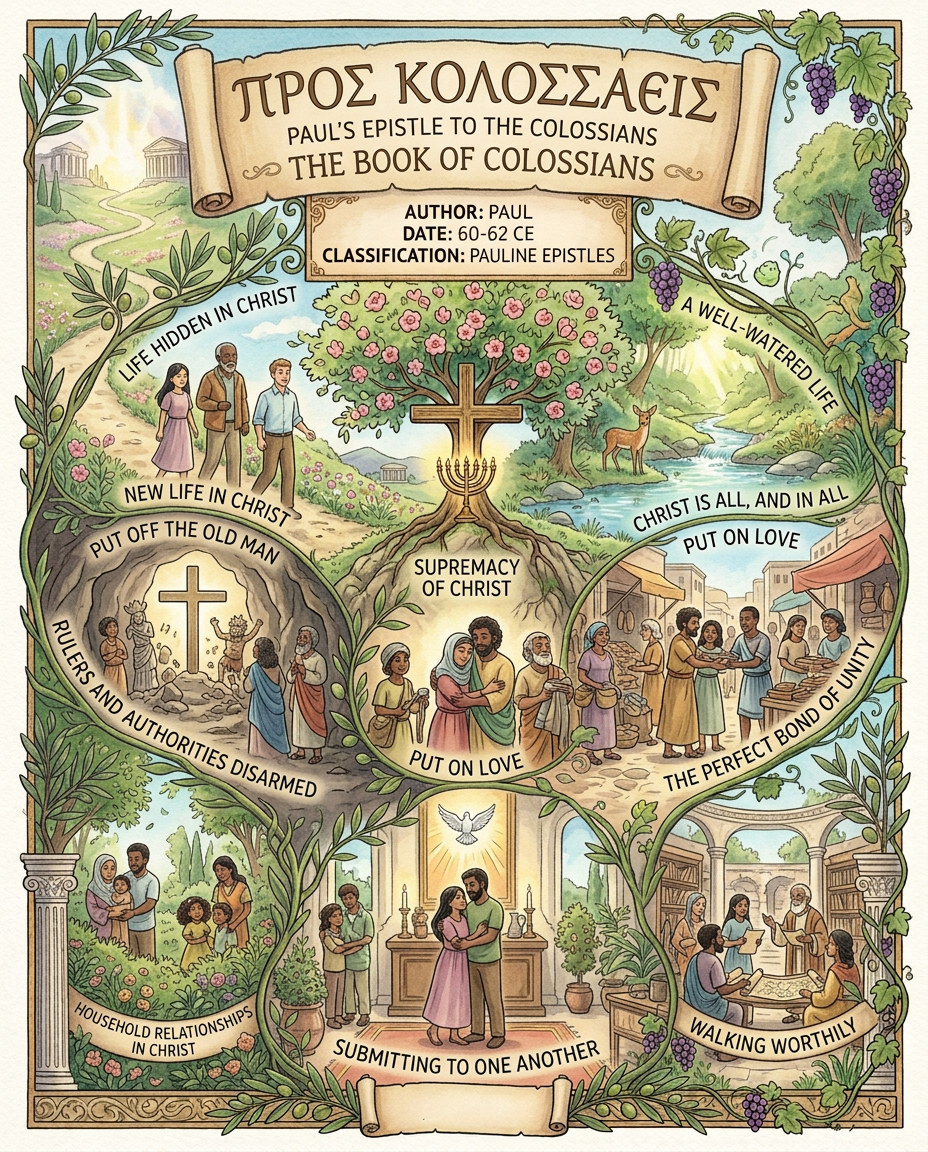
\includepdf[pages=1, fitpaper=false, width=\paperwidth, height=\paperheight, , keepaspectratio=false]{images/divider2/colossians2.png}
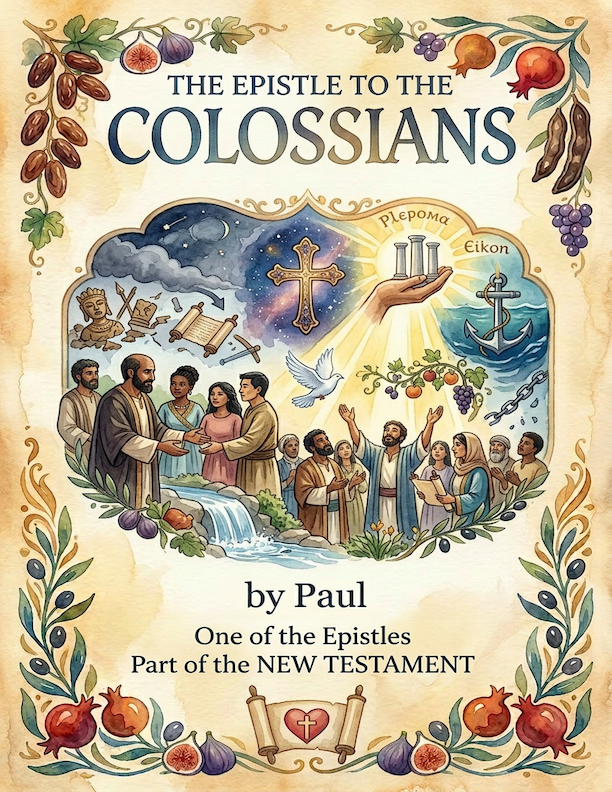
\includepdf[pages=1, fitpaper=false, width=\paperwidth, height=\paperheight, , keepaspectratio=false]{images/divider1/colossians.png}

\includepdf[pages=1, fitpaper=false, width=\paperwidth, height=\paperheight, , keepaspectratio=false]{images/8.5x11-Dot-Grid.png}

\includepdf[pages=1, fitpaper=false, width=\paperwidth, height=\paperheight, , keepaspectratio=false]{images/8.5x11-Dot-Grid.png}

\mybook{Colossians}
\vspace{-1.36in}


\mychapter{} \myverse*{}Paul, an emissary of Messiah\footnote{1:1 “Messiah” means “Anointed One”.} Yeshua through the will of God, and Timothy our brother,
\myverse{}to the holy ones and faithful brothers\footnote{1:2 The word for “brothers” here and where context allows may also be correctly translated “brothers
	and sisters” or “siblings.”} in Messiah at Colossae: Grace to you and peace from God our Father
and the Lord Yeshua the Messiah.

\myverse{}We give thanks to God the Father of our Lord Yeshua the Messiah,
praying always for you,
\myverse{}having heard of your faith in Messiah Yeshua and of the love which you have
toward all the holy ones,
\myverse{}because of the hope which is laid up for you in the heavens, of which you heard
before in the word of the truth of the Good News
\myverse{}which has come to you, even as it is in all the world and is bearing fruit and
growing, as it does in you also, since the day you heard and knew the grace of God in truth,
\myverse{}even as you learned from Epaphras our beloved fellow servant, who is a faithful
servant of Messiah on your\footnote{1:7 NU reads \textit{our}} behalf,
\myverse{}who also declared to us your love in the Spirit.

\myverse{}For this cause, we also, since the day we heard this, don’t cease
praying and making requests for you, that you may be filled with the knowledge of his will in all spiritual
wisdom and understanding,
\myverse{}that you may walk worthily of the Lord, to please him in all respects, bearing
fruit in every good work and increasing in the knowledge of God,
\myverse{}strengthened with all power, according to the might of his glory, for all
endurance and perseverance with joy,
\myverse{}giving thanks to the Father, who made us fit to be partakers of the inheritance
of the holy ones in light,
\myverse{}who delivered us out of the power of darkness, and translated us into the
Kingdom of the Son of his love,
\myverse{}in whom we have our redemption,\footnote{1:14 TR adds “through his blood,”
} the forgiveness of our sins.

\myverse{}He is the image of the invisible God, the firstborn of all creation.
\myverse{}For by him all things were created in the heavens and on the earth, visible
things and invisible things, whether thrones or dominions or principalities or powers. All things have
been created through him and for him.
\myverse{}He is before all things, and in him all things are held together.
\myverse{}He is the head of the body, the assembly, who is the beginning, the firstborn
from the dead, that in all things he might have the preeminence.
\myverse{}For all the fullness was pleased to dwell in him,
\myverse{}and through him to reconcile all things to himself by him, whether things
on the earth or things in the heavens, having made peace through the blood of his cross.

\myverse{}You, being in past times alienated and enemies in your mind in
your evil deeds,
\myverse{}yet now he has reconciled in the body of his flesh through death, to present
you holy and without defect and blameless before him,
\myverse{}if it is so that you continue in the faith, grounded and steadfast, and not
moved away from the hope of the Good News which you heard, which was proclaimed in all creation under
heaven, of which I, Paul, was made a servant.

\myverse{}Now I rejoice in my sufferings for your sake, and fill up on
my part that which is lacking of the afflictions of Messiah in my flesh for his body’s sake, which is
the assembly,
\myverse{}of which I was made a servant according to the stewardship of God which was
given me toward you to fulfill the word of God,
\myverse{}the mystery which has been hidden for ages and generations. But now it has
been revealed to his holy ones,
\myverse{}to whom God was pleased to make known what are the riches of the glory of
this mystery among the Gentiles, which is Messiah in you, the hope of glory.
\myverse{}We proclaim him, admonishing every man and teaching every man in all wisdom,
that we may present every man perfect in Messiah Yeshua;
\myverse{}for which I also labor, striving according to his working, which works in
me mightily.


% COLOSSIANS
\mychapter{} \myverse*{}For I desire to have you know how greatly I struggle for you and
for those at Laodicea, and for as many as have not seen my face in the flesh;
\myverse{}that their hearts may be comforted, they being knit together in love, and gaining
all riches of the full assurance of understanding, that they may know the mystery of God, both of the
Father and of Messiah,
\myverse{}in whom all the treasures of wisdom and knowledge are hidden.
\myverse{}Now I say this that no one may delude you with persuasiveness of speech.
\myverse{}For though I am absent in the flesh, yet I am with you in the spirit, rejoicing
and seeing your order, and the steadfastness of your faith in Messiah.

\myverse{}As therefore you received Messiah Yeshua the Lord, walk in him,
\myverse{}rooted and built up in him and established in the faith, even as you were taught,
abounding in it in thanksgiving.

\myverse{}Be careful that you don’t let anyone rob you through his philosophy
and vain deceit, after the tradition of men, after the elemental spirits of the world, and not after Messiah.
\myverse{}For in him all the fullness of the Deity dwells bodily,
\myverse{}and in him you are made full, who is the head of all principality and power.
\myverse{}In him you were also circumcised with a circumcision not made with hands,
in the putting off of the body of the sins of the flesh, in the circumcision of Messiah,
\myverse{}having been buried with him in immersion, in which you were also raised with
him through faith in the working of God, who raised him from the dead.
\myverse{}You were dead through your trespasses and the uncircumcision of your flesh.
He made you alive together with him, having forgiven us all our trespasses,
\myverse{}wiping out the handwriting in ordinances which was against us. He has taken
it out of the way, nailing it to the cross.
\myverse{}Having stripped the principalities and the powers, he made a show of them
openly, triumphing over them in it.

\myverse{}Let no one therefore judge you in eating or drinking, or with
respect to a feast day or a new moon or a Sabbath day,
\myverse{}which are a shadow of the things to come; but the body is Messiah’s.
\myverse{}Let no one rob you of your prize by self-abasement and worshiping of the angels,
dwelling in the things which he has not seen, vainly puffed up by his fleshly mind,
\myverse{}and not holding firmly to the Head, from whom all the body, being supplied
and knit together through the joints and ligaments, grows with God’s growth.

\myverse{}If you died with Messiah from the elemental spirits of the world,
why, as though living in the world, do you subject yourselves to ordinances,
\myverse{}“Don’t handle, nor taste, nor touch”
\myverse{}(all of which perish with use), according to the precepts and doctrines of
men?
\myverse{}These things indeed appear like wisdom in self-imposed worship, humility,
and severity to the body, but aren’t of any value against the indulgence of the flesh.


% COLOSSIANS 3
\mychapter{} \myverse*{}If then you were raised together with Messiah, seek the things
that are above, where Messiah is, seated on the right hand of God.
\myverse{}Set your mind on the things that are above, not on the things that are on the
earth.
\myverse{}For you died, and your life is hidden with Messiah in God.
\myverse{}When Messiah, our life, is revealed, then you will also be revealed with him
in glory.

\myverse{}Put to death therefore your members which are on the earth: sexual
immorality, uncleanness, depraved passion, evil desire, and covetousness, which is idolatry.
\myverse{}For these things’ sake the wrath of God comes on the children of disobedience.
\myverse{}You also once walked in those, when you lived in them,
\myverse{}but now you must put them all away: anger, wrath, malice, slander, and shameful
speaking out of your mouth.
\myverse{}Don’t lie to one another, seeing that you have put off the old man with his
doings,
\myverse{}and have put on the new man, who is being renewed in knowledge after the image
of his Creator,
\myverse{}where there can’t be Greek and Jew, circumcision and uncircumcision, barbarian,
Scythian, bondservant, or free person; but Messiah is all, and in all.

\myverse{}Put on therefore, as God’s chosen ones, holy and beloved, a heart
of compassion, kindness, lowliness, humility, and perseverance;
\myverse{}bearing with one another, and forgiving each other, if any man has a complaint
against any; even as Messiah forgave you, so you also do.

\myverse{}Above all these things, walk in love, which is the bond of perfection.
\myverse{}And let the peace of God rule in your hearts, to which also you were called
in one body, and be thankful.
\myverse{}Let the word of Messiah dwell in you richly; in all wisdom teaching and admonishing
one another with psalms, hymns, and spiritual songs, singing with grace in your heart to the Lord.

\myverse{}Whatever you do, in word or in deed, do all in the name of the Lord Yeshua,
giving thanks to God the Father through him.

\myverse{}Wives, be in subjection to your husbands, as is fitting in the
Lord.

\myverse{}Husbands, love your wives, and don’t be bitter against them.

\myverse{}Children, obey your parents in all things, for this pleases the
Lord.

\myverse{}Fathers, don’t provoke your children, so that they won’t be discouraged.

\myverse{}Servants, obey in all things those who are your masters according
to the flesh, not just when they are looking, as men pleasers, but in singleness of heart, fearing God.
\myverse{}And whatever you do, work heartily, as for the Lord and not for men,
\myverse{}knowing that from the Lord you will receive the reward of the inheritance;
for you serve the Lord Messiah.
\myverse{}But he who does wrong will receive again for the wrong that he has done, and
there is no partiality.


% COLOSSIANS 4
\mychapter{} \myverse*{}Masters, give to your servants that which is just and equal, knowing
that you also have a Master in heaven.

\myverse{}Continue steadfastly in prayer, watching in it with thanksgiving,
\myverse{}praying together for us also, that God may open to us a door for the word, to
speak the mystery of Messiah, for which I am also in bonds,
\myverse{}that I may reveal it as I ought to speak.

\myverse{}Walk in wisdom toward those who are outside, redeeming the time.
\myverse{}Let your speech always be with grace, seasoned with salt, that you may know
how you ought to answer each one.

\myverse{}All my affairs will be made known to you by Tychicus, the beloved
brother, faithful servant, and fellow bondservant in the Lord.
\myverse{}I am sending him to you for this very purpose, that he may know your circumstances
and comfort your hearts,
\myverse{}together with Onesimus, the faithful and beloved brother, who is one of you.
They will make known to you everything that is going on here.

\myverse{}Aristarchus, my fellow prisoner, greets you, and Mark the cousin
of Barnabas (concerning whom you received instructions, “if he comes to you, receive him”),
\myverse{}and Yeshua who is called Justus. These are my only fellow workers for God’s
Kingdom who are of the circumcision, men who have been a comfort to me.

\myverse{}Epaphras, who is one of you, a servant of Messiah, salutes you,
always striving for you in his prayers, that you may stand perfect and complete in all the will of God.
\myverse{}For I testify about him that he has great zeal for you, and for those in Laodicea,
and for those in Hierapolis.
\myverse{}Luke the beloved physician and Demas greet you.
\myverse{}Greet the brothers who are in Laodicea, with Nymphas and the assembly that
is in his house.
\myverse{}When this letter has been read among you, cause it to be read also in the
assembly of the Laodiceans, and that you also read the letter from Laodicea.
\myverse{}Tell Archippus, “Take heed to the ministry which you have received in the
Lord, that you fulfill it.”

\myverse{}I, Paul, write this greeting with my own hand. Remember my chains.
Grace be with you. Amen.


